\documentclass[../main/main.tex]{subfiles}

\newdate{date}{3}{12}{2020}


\begin{document}

\chapter{Model fitting}
\marginpar{ \textbf{Lecture 19.} \\  \displaydate{date}. \\ Compiled:  \today.}

The next step one must make is now \textbf{make sense} of data. Therefore, we want to \textbf{extract meaningful information} out of it by the mean of a model. However, there are also many \textbf{challenges} when collecting data: one should think well about what kind of data is needed, as well as the measurement process and its interpretation. We are going to analyze these arguments using as paradigmatic example COVID-19, but our considerations can actually be applied to \textit{any} spread process.

\section{Data Collection}

When dealing with epidemic processes one usually speaks about \textbf{incidence data}, like the one depicted in figure \ref{fig:19_01}.

\begin{figure}[h!]
\centering
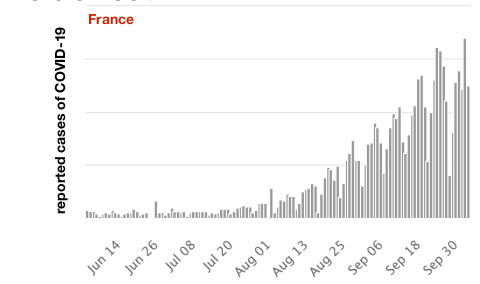
\includegraphics[width=0.8\textwidth]{../lessons/image/19/image01.png}
\caption{\label{fig:19_01} COVID-19 curve incidence data in France. For each day, number of reported new cases are shown.}
\end{figure}

We want to \textbf{model} these data, so in other words we want to make \textbf{make sense} out of it by interpreting raw numbers. In order to do it, we need first to understand how it was collected and, recalling that data actually gives \textbf{partial information}, this must be \textit{completed} by the means of a \textbf{model}.

The main \textbf{goals} one wants to pursue by using models are:
\begin{itemize}
    \item \textbf{nowcasting}: provide assessment regarding the \textit{present} and \textit{close future} of the epidemics. Therefore, one may need to understand what is and what will be the extension/distribution by groups/regions of the epidemic that is present at that moment, given the partial information returned by data.
    \item \textbf{forecasting}: prediction in \textit{longer term}. For instance, one would like to predict hospitals occupancy, when and how high will be the epidemic peak, how many people will be infected over the next weeks or months, when epidemic will end and what will be its final size.
    \item \textbf{medical and biological understanding}: at the very beginning we have no medical/biological knowledge about the epidemic. Hence, we want to study for instance how it propagates and through what vectors (human-to-human, zoonotic, vector-borne, direct transmission, fomite, aerosol, droplets, etc...), the role of asymptomatic/pre-symptomatic in transmission, susceptibility and rate of symptoms by age group.
    \item \textbf{exploration of counterfactuals and hypothetical scenarios}: we run our model to perform \textit{scenario analysis} and understand what is the best strategy to use in the future. It may be related to vaccination, pharmacological interventions, lockdown, travel restrictions and their impact on the future spreading. Indeed, these are \textit{long-term} projections, despite one may want to explore the case and what would have occurred if a decision had not been made. Hence these arguments are valid also for the past: for instance we want to quantify the impact of lockdown in spreading.
\end{itemize}

Let us discuss \textbf{what} is the \textit{data} we usually work with. When we speak about \textbf{incidence in a given area and at time} $t$, we refer to the \textbf{fraction} of population resident in that area that has contracted the disease at time $t$. Hence, formalizing\footnote{We will use \textit{flu} as example, since we have much data of it}:
\begin{equation}
    \text{\textbf{incidence}} = \frac{\text{number of people hit by flu}}{\text{population at risk}}
\end{equation}
Let us take a look closer to the \textbf{numerator}. Obviously it is impossible to have a complete information about how many people have the flu at this moment. But, first, one has to face the first problem of \textbf{case definition}: set of criteria used in making a decision as to whether an individual has a disease or any other health event of interest. Some possible \textit{criteria} may involve: clinical (e.g. symptoms), laboratory characteristics (e.g. exams, test results). Moreover personal information are taken into account, such as whether this individual travelled to regions at risk/had contact with people at risk can be classified using three levels: confirmed, probable, possible. Cases definition can be either more \textit{sensitive} or \textit{specific}, and it has to be tuned according to the risk assessment. A \textbf{sensitive} case definition will detect many cases but may also count as cases individuals who do not have the disease (\textit{possible overestimation}). On the other hand, \textbf{specific} case definition is more likely to include only persons who truly have the disease under investigation but also more likely to miss some cases (\textit{possible underestimation}). This is summarized in Fig. \ref{fig:19_02}.

\begin{figure}[h!]
\centering
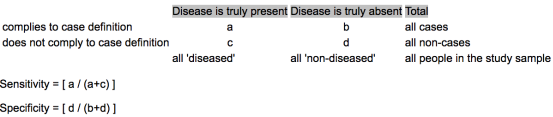
\includegraphics[width=0.9\textwidth]{../lessons/image/19/image02.png}
\caption{\label{fig:19_02} Case definition can be either more sensitive or specific. In the first case we may end up overestimating the number of cases, whereas when a test is more specific this might lead to underestimation.}
\end{figure}

Let us see \textbf{how} data is \textbf{collected}: in France there is a network of \textit{General Practitioners} (see Fig. \ref{fig:19_04}) that are volunteers and daily send a report to Health Minister concerning all the cases they have visited during a workday. However, for some diseases, for instance measles, every family doctor is obliged to report the case. Let us continue analyzing the \textit{flu} case. The number of cases reported is indeed the number of cases seen by General Practitioners defined under the basis of some clinical criteria. These are \textit{possible cases}: the guarantee can be returned only after a laboratory confirmation which is available only for a small proportion of cases.

\begin{figure}[h!]
\centering
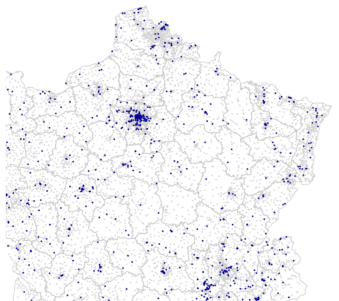
\includegraphics[width=0.6\textwidth]{../lessons/image/19/image04.png}
\caption{\label{fig:19_04} The Surveillance Network in france $(SN)$ is based on a fraction of General Practitioner ($\sim1\%$), who are volunteers.}
\end{figure}

Given the symptoms of flu:
\begin{itemize}
\item no symptoms (\( \sim 30 \% \));
\item upper respiratory symptoms, e.g. nasal stuffiness, runny nose, sore throat, sneezing, hoarseness, ear pressure, or earache (\( \sim 60 \% \));
\item lower respiratory symptoms, e.g. cough, breathing difficulty, and chest discomfort (\( \sim 2 \% \));
\item fever (\( \sim 35 \% \));
\end{itemize}
The main concept is that it is important to understand according to what criteria data is collected in order to deal better with observables, indeed observables are a \textit{proxy} for the real data.
One should note that they may be different even if they regard the same quantity (look Fig. \ref{fig:19_03_sub}): for $ECDC$ incidence data we might observe a peak in autumn because of respiratory infections, whereas this might not be present in $Sentinelles$ reports, given they do not classify it as case of flu. The $ECDC$ case definition, as one can imagine, has higher sensitivity and this can return overestimation of the number of cases. Conversely, according to $Sentinelles$ cases definition we might underestimate their number.

\begin{figure}[h!]
\begin{minipage}[]{0.5\linewidth}
\centering
\subfloat[]["Sentinelles" clinical case definition for flu.]{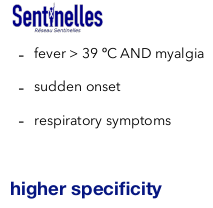
\includegraphics[width=0.9\textwidth]{../lessons/image/19/image03b.png}  \label{fig:} }
\end{minipage}
\begin{minipage}[]{0.5\linewidth}
\centering
\subfloat[]["ECDC" clinical case definition for flu.]{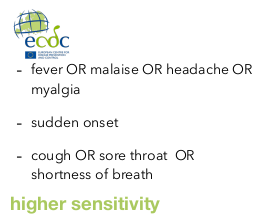
\includegraphics[width=0.9\textwidth]{../lessons/image/19/image03c.png}  \label{fig:} }
\end{minipage}
\caption{\label{fig:19_03_sub} }
\end{figure}




Let us take a look closer to the \textbf{denominator}. It refers to the \textit{catchment population}, i.e. all the people living
in the catchment area of the General Practitioner reporting the cases, who would usually seek healthcare at the site when they get sick. Therefore, the denominator for the area \( a \) that can be computed at a first approximation is\footnote{Horvitz DG, Thompson DJ. A JASA. 1952;47:663–85}:
\begin{equation*}
    \text{denominator}_a = \text{Population}_a \frac{GP_{SN,a}}{GP_a}
\end{equation*}
where the ratio $\frac{GP_{SN,a}}{GP_a}$ is the proportion of General Practitioners that contribute to the \textit{Surveillance Network} ($\sim1\%$ according to Fig. \ref{fig:19_04}). Moreover, another \textbf{problem} that biases our observable is given by the \textbf{consultancy rate}. Since many people are asymptomatic or paucisymptomatic, the rate of people going to be examinated by family doctor is highly variable by age: young people, except very little children, are more likely to not go, whereas adults need to go in order to have permission to stay home from work. Raw numbers depend also on family doctors density, on the health-care system (how expensive is going to the GP), and on the period of the year that brings specific diseases. In conclusion, even though data might look simple at a first glance, dealing with it needs to take into account many variables all together and some assumptions are more likely to be made if data is not available. Another important point is that the \textbf{confirmed flu cases} are a very small subset among \textit{I}nfluenza \textit{L}ike \textit{I}lness $(ILI)$ people (symptomatic), people that go to General Practitioner, Infected people which either can be detectable or not and that, obviously, need to be recorded as infected.

Another \textit{characteristic} of the \textbf{case definition} is that it might be \textbf{variable in time}, specially when the range of symptoms is still unknown. It was the case of \textbf{COVID-19} at the very beginning. In addition, case definition is \textbf{matter of authority}: once cases are reported in hospitals, some papers concerning viral loads, symptoms, evidences are published. Health authority needs to collect and through them in order to define better the case definition, keeping in mind a sort of trade off: if case definition is \textit{high sensitive}, there might be false positives and also cause panic among people. Conversely, if the definition is \textit{too much specific}, we risk to let infectious people go around and spread the infection. This tuning depends on the goals one may want to pursue.

With regards to \textbf{COVID-19}, case definition was therefore varying in time being the range of symptoms unknown. Moreover, more problems arose since the disease at the \textit{very beginning} was not wide spread and it was still unclear the region where it was spreading: the denominator related to the catchment population was kind of difficult to estimate at that time. The \textit{reporting rate} was highly variable in time: at the beginning, the tracing system is able to intercept all the case, but the surveillance system might saturate even though the case definition remains unchanged. Moreover, due to the change in time of case definition, number of cases can be always retrospectively corrected: real time analysis numbers are indeed biased and this is why sometimes we observe spikes in incidence curves.






\section{Epidemic Modeling and Bayesian Inference}

Typically, the steps are the following ones:
\begin{itemize}
    \item \textbf{Model design/implementation}: decide the model ingredients that synthesise available medical, biological, information etc. We can consider different models, ingredients that describe our \textbf{hypotheses}. These can be for instance helpful to simplify our problem and must be \textit{clearly} stated at the beginning.
    \item \textbf{Model calibration}: estimate model parameters from available data, a.k.a. model \textit{fitting}
    \item \textbf{Model validation}: confirming that model output is sufficiently accurate in reproducing the data. It is done as the result of \textit{model calibration}, when we can tell whether our model well represents data also taking into account secondary aspects.
\end{itemize}

Let us introduce now some concepts about \textbf{bayesian inference} and \textbf{Maximum Likelihood} that will help us throughout this process. Once we observe data, one wants to introduce an \textbf{Observation model} $\mathcal{O}$ according to which we assume to have acquired our data. In our case, we assume it to be a \textit{Binomial} process with probability $p$: every case, according to a probability $p$ goes to the doctor. In addition we need to define an \textbf{Epidemic Model} (e.g. $SIR$, or alternatively $SEIR$, $SIRS$...) and a \textbf{vector of parameters} $\vec{\theta} = ( \beta, \mu, ...)$ where some are to be inferred, while others are assumed to kept fixed. This obviously depends on our data and on our \textbf{Initial Conditions} $I_0$, namely the number of infectious. All these quantities help us to define the curve represented in Fig.\ref{fig:19_05}.

\begin{figure}[h!]
\centering
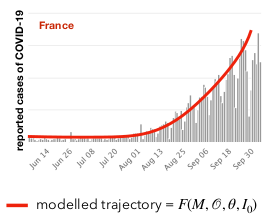
\includegraphics[width=0.6\textwidth]{../lessons/image/19/image05.png}
\caption{\label{fig:19_05} Curve fitting the incidence curve presented before (see Fig. \ref{fig:19_01}). }
\end{figure}

We therefore use a \textbf{Maximum Likelihood approach} that returns from a probabilistic formulation: indeed the relation between model and data is probabilistic, and our aim is to  identify the trajectory and thus the parameters, $\vec{\theta}$, that are \textbf{more probable given the data} we have. One should note that, in the \textit{bayesian framework} probability is used as a \textbf{measure of uncertainty}.

When we are dealing with single random variable $A$ we talk about \textit{univariate probability}: the probability that $A$ takes value $a$ is defined as $p(A=a)=p(a)$ and the normalization condition holds $\sum_a p(a) = 1$. For \textit{continuous variables} it can be rewritten as  $\int p(a)\dd[]{a}= 1$. When random variables are more than one, e.g. $A$, $B$, the joint probability that $A$ takes value $a$ and $B$ takes value $b$ is written as $p(A=a,B=b) = p(a,b)$. The marginal probability $p(a) = \sum_b p(a,b)$ and is the probability that $A$ takes value $a$ regardless $b$: we indeed summed over all the possible $p(b)$.
For \textit{continuous variables} it can be rewritten as $p(a) = \int p(a,b,)db$

Some of the \textbf{basic properties} we will deal are the following:
\begin{itemize}
    \item \textbf{Conditional probability} of $a$ from random variable $A$, given that the outcome of a random variable $B$ was $b$ is $p(A=a|B=b) = p(a|b)$.
    \item \textbf{Bayes Theorem} allows us to rewrite the conditional probability as follows $p(a|b) = \frac{p(a,b)}{p(b)}$.
    \item \textbf{Chain rule}: $p(a,b,c) = p(a|b,c)p(b|c)p(c)$.
\end{itemize}

We are going now to introduce some variables and a short overview over statistical inference. As said, the latter helps us in drawing conclusions from numerical data about quantities that are not observed: for instance we see that a disease is more frequent in adults and we want to infer its prevalence in children population. Some of these unobserved quantities can be $\mathbf{\Tilde{y}}$: potentially observable quantities such as future observations of a process (e.g. predictions), and $\mathbf{\vec{\theta}}$ that are quantities not directly observable such as \textit{parameters} that govern hypothetical process. \textbf{Bayesian statistical conclusions} about a parameter $\theta$ or unobserved data $\Tilde{y}$ are made in terms of \textit{probability statements}. These are expressed as \textbf{conditional} probabilities on the observed values of $y$: $p(\theta|y)$.

In other words, we want to obtain a distribution for $\theta$ conditioned to $y$: $p(\theta|y)$. In order to pursue our goal:
\begin{itemize}
    \item we need a model $(M)$ that provides us the joint probability distribution of $\theta$ and $y$: $p(\theta, y)$;
    \item given the model $M$, thanks to Bayes' Theorem we can write $p(\theta,y) = p(y|\theta)p(\theta)$, with $p(\theta)$ that is the \textbf{prior distribution} and $p(y|\theta)$ that is the sampling distribution;
    \item we use the Bayes rule to \textit{condition} on the known value of the data $y$, namely:
    \begin{equation*}
        p(\theta,y) = p(\theta|y)p(y) = p(y|\theta)p(\theta)
    \end{equation*}
\end{itemize}
The \textbf{unnormalized posterior density}, namely the expression that helps us inferring the parameters we need, is:
\begin{equation}
    p(\theta|y) \propto p(\theta) p(y|\theta)
\end{equation}
It is unnormalized since we do not care about the normalization term: it is constant.

One should note that data affects the posterior \textbf{only} through $p(y|\theta)$. If we keep fixed $y$ and let $\theta$ vary, this is the \textbf{Likelihood function} $\mathcal{L}(\theta) = p(y|\theta)$


\begin{example}{Hemophilia}{}

Let us consider now an \textbf{example}. \textit{Hemophilia} is a hereditary disease associated to a gene of the chromosome $X$. This is recessive inheritance: a man who inherits the gene is affected, a woman who inherits the gene on only one X is not affected. Let us recall, for the sake of completeness, that a man has chromosomes $XY$, while woman $XX$.

We want to deal with the following \textbf{problem}: given that a woman has an affected brother and a father not affected, she can be a carrier of the gene on either one $X$. We want to estimate whether she is a carrier, and we define $\theta = 1$ as the situation where she actually is, while $\theta = 0$ describes a situation where she is not. Since we do not have \textit{any} other information, \textbf{a priori} one should not introduce any bias, hence $p(\theta = 1 ) = p(\theta = 0) = 0.5$.

Our empirical \textbf{data} consists on the fact that she has got two sons, and neither of the two is affected: $y_1 = 0$ and $y_2=0$. The \textbf{Likelihood} is therefore:
\begin{align*}
    p(y_1 = 0, y_2 = 0 | \theta = 1 )&= 0.5^2\\
    p(y_1 = 0, y_2 = 0 | \theta = 0 )&= 1
\end{align*}

Multiplying these terms, we can obtain the \textbf{posterior}, namely:
\begin{equation*}
\begin{split}
    p(\theta = 1 | y_1, y_2) &= \frac{p( y_1, y_2 | \theta = 1)p(\theta = 1)}{p( y_1, y_2 | \theta = 1)p(\theta = 1)+ p( y_1, y_2 | \theta = 0)p(\theta = 0)} \\ &= \frac{0.25 \cdot 0.5}{0.25 \cdot 0.5 + 0.5} = 0.2
\end{split}
\end{equation*}
So the probability that she is a carrier, given our observation is quite low.

However, most of the times, it might happen that \textbf{new data is available}: for example the same woman has a third son, which is not affected $y_3 = 0$. Obviously, one does not want to lose all the information obtained so far, hence we \textbf{update the prior}. The \textbf{prior} becomes:
\begin{equation*}
    p(\theta = 1 ) = 0.2, \qquad p(\theta = 0) = 0.8
\end{equation*}
which is the posterior of before.
The \textbf{Likelihood} follows the same argument as before $P(y_3 = 0 | \theta = 1 ) = 0.5$. Out of these expression we can compute the \textbf{posterior}, which is:
\begin{align*}
        p(\theta = 1 | y_3) = \frac{p(  y_3 | \theta = 1)p(\theta = 1)}{p(  y_3 | \theta = 1)p(\theta = 1)+ p(  y_3 | \theta = 0)p(\theta = 0)} = \frac{0.5 \cdot 0.2}{0.5 \cdot 0.2 + 0.8} = 0.111
\end{align*}
Indeed, the probability for the woman to be a carrier is even lower. We want to stress once again that, updating the posterior, we have not lost any information that was previously obtained.

\end{example}


\begin{example}{Bernoulli trial}{}
Let us consider \textbf{another example}, with \textit{Bernoulli trials}. Recalling that for a \textbf{Binomial distribution} we have $n$ independent trials with two possible complementary outcomes (either failure or success) and we observe $y$ successes. The probability of a success is $\theta$, consequently for a failure is $1-\theta$ and this is the parameter one may want to estimate. For instance, given a number $n$ of observations with $y$ successes, we want to infer whether a coin is fair $\theta = 1/2$.

In the case, we do not have any information so we can use a \textbf{uniform prior} for the paramter$\theta$: $\mathcal{U}[0,1]$. The \textbf{Likelihood} is a \textit{Binomial distribution} with parameters:
\begin{equation*}
P(y|\theta) = \texttt{Bin}(y|n,\theta ) = \binom{n}{y} \theta^y (1-\theta)^{n-y}
\end{equation*}
Note as we do not write the dependence on $n$ on the left side because is part of the experimental design and considered fixed. All probabilities will be conditional on $n$. The \textbf{posterior} becomes:
\begin{equation*}
    p(\theta|y) \propto \theta^y (1-\theta)^{n-y}
\end{equation*}
that is nothing more that a \textit{Beta} distribution $\text{Beta}(y+1, n-y+1)$. Note that $\binom{n}{y}$ does not depend on $\theta$ therefore can be disregarded.

\end{example}

\begin{figure}[h!]
\centering
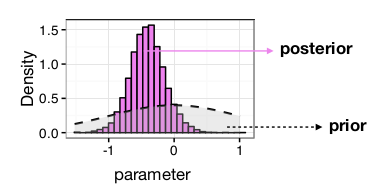
\includegraphics[width=0.45\textwidth]{../lessons/image/19/image06.png}
\caption{\label{fig:19_06} When we work with Bayesian inference we usually want to infer the most likely value for a parameter thanks to the \textit{posterior}, given the observation (\textit{data}) and our previous knowledge (\textit{prior}). }
\end{figure}

Shortly, the \textbf{prior distribution} summarises my a priori knowledge about parameters. It might be defined based on the literature, for instance if we are analysing an outbreak of flu and our goal is to estimate $R_0$, we may want to look at previous $R_0$ estimates. If we have no prior knowledge on the problem, however, the best idea is to use a vague, or flat, \textit{noninformative} prior. Instead, the \textbf{posterior distribution} is a compromise between data and prior information. Such compromise is increasingly controlled by data as the sample size increases. Posterior \textit{variance} on average is smaller than prior variance: if it occurs, then this denotes either a conflict or an inconsistency between sampling model (i.e. data we obtain) and the prior distribution. The \textbf{main information} one wants to obtain from the posterior are:
\begin{itemize}
    \item \textbf{Mode} of the posterior, i.e. the most likely parameter given the data.
    \item \textbf{Uncertainty} associated to our estimate, i.e. the $C.I.$ (credibility interval) and usually it is given by the $2.5\%$ and $97.5\%$ quantiles. It is really a relevant quantity: the range according to which the mode spans can lead to really \textbf{different} and \textbf{opposite outcomes}.
\end{itemize}


\begin{figure}[h!]
\begin{minipage}[c]{0.3\linewidth}
\subfloat[][Raw data: incidence curve.]{ 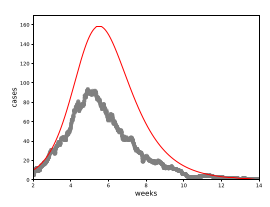
\includegraphics[width=0.8\textwidth]{../lessons/image/19/image07a.png}  \label{fig:19_07a} }
\end{minipage}
\hfill
\begin{minipage}[]{0.3\linewidth}
\centering
\subfloat[][Prediction of \textit{total} number of cases for $\theta = 0.36$, i.e. $I(t)$.]{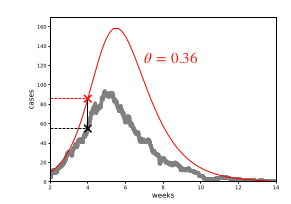
\includegraphics[width=0.8\textwidth]{../lessons/image/19/image07b.png}  \label{fig:19_07b} }
\end{minipage}
\hfill
\begin{minipage}[]{0.3\linewidth}
\centering
\subfloat[][Prediction of \textit{detected} number of cases for $\theta = 0.36$ at fourth week, i.e. $y_{t=4}$.]{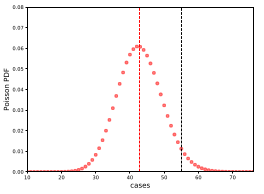
\includegraphics[width=0.8\textwidth]{../lessons/image/19/image07c.png}  \label{fig:} }
\end{minipage}
\caption{\label{fig:19_07c} }
\end{figure}


Let us discuss now a more practical problem. We want now to understand how to \textbf{fit an incidence curve}, such as the one in Fig. \ref{fig:19_07a} where all symptomatic cases that go to the doctor are detected, to estimate $R_0$. In other words, we have an incidence curve and want to fit a $SIR$ model. The steps to follow are:
\begin{itemize}
    \item \textbf{Data}. We know that the infection causes \textit{symptoms} for the $50\%$ of cases. We assume that all symptomatic cases go to the doctor and are detected.
    \item \textbf{Observation model}: weekly cases are independently detected with probability $d = 0.5$. Observations $y_t$ are independent. This process is binomial: each case has the $50\%$ to be detected. However, for large numbers, it can be approximated as a Poisson.
    \item \textbf{Model}: SIR, from the literature and peer review journals we know that the average infection duration is $\mu^{-1} = 5.5$ days. We can assume this parameters to be fixed.
    \item \textbf{Parameter} we want to fit is $\theta = \beta$
    \item \textbf{Prior} uniform in $[0,1]$, since we do not have any information on $\beta$.
    \item \textbf{Likelihood} $\mathcal{L}(\theta) = p(y_1, ,...y_t,...,y_{t_M}|\theta) = \prod_t p(y_t|\theta)$, cases at $t$-th week are denoted by $y_t$
\end{itemize}

Then, for each value of $\beta$ (our $\theta$ to be inferred) we run a simulation of the trajectory of the $SIR$, fixing $\mu$ and $I_0$ based on available knowledge.
Practically, we can approximate observed data to be distributed as a $\text{Poisson}(\lambda)$, where $\lambda = I(t)d$. This is the number of cases we see at $t$-th week times the detection probability. The total number of cases is distributed as the red line in fig. \ref{fig:19_07b}. This returns us the model projection related to the observation.

For instance, at week $t = 4$, we observe $y_{t=4} = 55$ cases. If we assume data is distributed as a Poisson, the sampling distribution is $y_{t=4}|\theta \sim \text{Poisson}(\lambda)$, then $\lambda = I(t) d = 86\cdot 0.5 = 43$ we expect $43$ detected cases. Keeping the parameter $\theta$ fixed, we have to compute the likelihood as $\mathcal{L}(\theta = 0.36) = \text{Poisson}(55|\lambda)$. This procedure has to be done for every value of the parameter $\theta$. Moreover, one should take into account that since dealing with products is uncomfortable because of really small numbers and for computational simplicity, we take the logarithm\footnote{It can be done since $\mathcal{L}(\theta)$ is monotone, without any losing of generality.} of the likelihood, therefore considering the sum: $\log \mathcal{L}(\theta) = \sum_t \log\ p(y_t|\theta)$.

Let us summarize the \textbf{basic idea} behind likelihood computation: we want to evaluate the probability of the data given the model and the parameters. In order to \textbf{estimate} $\theta$ we keep the model $M$ and $x_0$ fixed and vary $\theta$ to compute the probability $p(y|\theta)$. The Likelihood function is $\mathcal{L} (\theta) = p(y | \theta)$, and generally it can span a wide range of orders of magnitude, which can lead to numerical problems. In practice it is better to work with the log-likelihood: $\log \mathcal{L}(\theta) = \log\ p(y_1, ..., y_n | \theta) = \sum_i \log\ p (y_i | \theta)$. The best estimate for $\theta$ is actually the one that maximizes the posterior, i.e. the \textbf{mode}.


\end{document}
